\section{\ourapproach}
% \section{\tool: \underline{Cau}sal \underline{Per}formance Debugging}
\label{sec:methodology}
% \begin{figure}[t!]
    
    \begin{minipage}{\linewidth}
            \algcauper
        %     \caption{\small \tool framework.}
        \end{minipage}
        \\[-1em]
    %     \begin{minipage}{\linewidth}
    %             \algquery
    %             % \caption{\small Generating interventions.}
    % \end{minipage}
\end{figure}

% \begin{figure*}
%     \subfloat[][\tool]{
%         \begin{minipage}{0.5\linewidth}
%             \algcauper
%         \end{minipage}}
%     \subfloat[][Counterfactual query generation]{
%         \begin{minipage}{0.5\linewidth}
%             \algquery
%         \end{minipage}}
% \end{figure*}


This section presents \ourapproach--our methodology for performance analyses of highly configurable and composable systems with causal reasoning. 
%(e.g., DeepStream data analytics pipeline in \fig{deepstream_pipeline}). %First, we describe how we are expecting \tool to be used and provide a high-level overview of \tool. 

\smallskip
\begin{figure}[tp!]
    % \setlength{\belowcaptionskip}{-3em}
    \centering
    \includegraphics*[width=\linewidth]{UnicornOverview}
    \caption{\small {Overview of \ourapproach}.}
    % \vspace{-2em}
    \label{fig:overview}
    % \rayb{I have questions about this figure. Let's talk in the morning}
\end{figure}

\begin{figure}[tp!]
    % \setlength{\belowcaptionskip}{-3em}
    \centering
    \includegraphics*[width=\linewidth]{Config-Objective-Space-Mapping}
    \caption{\small {Mapping configuration space to multi-objective performance space.}}
    
    \label{fig:config_to_objective_space}
    \vspace{-4mm}
    % \rayb{I have questions about this figure. Let's talk in the morning}
\end{figure}
\paragraph{Overview.}
\ourapproach works in five stages, implementing an active learning loop (cf. \fig{overview}): (i) Users or developers of a highly-configurable system \emph{specify}, in a human-readable language, the performance task at hand in terms of a query in the Inference Engine. For example, a \textsc{Deepstream} user may have experienced a throughput drop when they have deployed it on NVIDIA Xavier in low-power mode (cf. \fig{config_to_objective_space}). Then, \ourapproach's main process starts by (ii) collecting some predetermined number of samples and \emph{learning a causal performance model}; Here, a sample contains a system configuration and its corresponding measurement—including low-level system events and end-to-end system performance. Given a certain budget, which in practice either translates to time~\cite{iqbal2020flexibo} or several samples~\cite{jamshidi2016uncertainty}, \ourapproach, at each iteration, (iii) \emph{determines the next configuration(s)} and measures system performance when deployed with the determined configuration--i.e. new sample; accordingly, (iv) the \emph{learned causal performance model is incrementally updated}, reflecting a model that captures the underlying causal structure of the system performance. \ourapproach terminates if either budget is exhausted or the same configuration has been selected a certain number of times consecutively, otherwise, it continues from Stage III. Finally, (v) to automatically derive the quantities which are needed to conduct the performance tasks, the specified performance queries are \emph{translated} to formal causal queries, and they will be \emph{estimated} based on the final causal model.

%  note that this translation is currently manual, however, afterward, (iii) the \emph{causal queries are estimated} in a query engine that employs the learned causal model and uses do-calculus to estimate the causal queries. In most cases, this involves estimating the causal effects of configuration options to performance objectives;

\begin{figure}[tp!]
    % \setlength{\belowcaptionskip}{-3em}
    \centering
    \includegraphics*[width=\linewidth]{Causal-Learning}
    \caption{\small {Causal model learning from performance data.}}
    
    \label{fig:causal_model_learning}
    % \rayb{I have questions about this figure. Let's talk in the morning}
\end{figure}


\smallskip
\noindent
\paragraph{Stage I: Formulate Performance Queries.}
\ourapproach enables ~\textit{developers} and ~\textit{users} of highly-configurable systems to conduct performance tasks, including performance debugging, optimization, and tuning, n particular, when they need to answer several performance queries:
%CK expand this a bit
%(Note about the format below...)
(i) What configuration options \emph{caused} the performance fault? (ii) What are \emph{important options and their interactions} that influence performance? (iii) How to \emph{optimize} one quality or navigate \textit{tradeoffs} among multiple qualities in a reliable and explainable fashion? (iv) How can we \emph{understand} what options and possible interactions are most responsible for the performance degradation in production? 
% How do we debug performance faults \emph{without direct access} to the user's deployment environment?
% How can I \emph{repair} the performance fault by changing the code that I am writing? 


\begin{figure}[tp!]
    % \setlength{\belowcaptionskip}{-3em}
    \centering
    \includegraphics*[width=\linewidth]{Causal-Model-Update}
    \caption{\small {Causal model update.}}
    
    \label{fig:causal_model_update}
    % \rayb{I have questions about this figure. Let's talk in the morning}
\end{figure}

At this stage, the performance queries are translated to formal causal queries using the interface of the causal inference engine (cf. \fig{overview}). Note that in the current implementation of \ourapproach, this translation is performed manually, however, this process could be made automated by creating a grammar for specifying performance queries and the translations can be made between the performance queries into the well-defined causal queries, note that such translation has been done in domains such as genomics~\cite{farahmand2019causal}.  %Finally, us are required to specify the initial number of samples, total budget (including the initial samples). 

% and translation of performance query to the associated causal queries in the query engine, so the quantities can be automatically estimated based on the learned causal model. 

% (note that the number of initial samples depends on the complexity of the system and the size of configuration space). 



% In a typical scenario, \ourapproach can be used when a developer experiences \nfps to (a)~identify which configuration options are the \textit{root causes} of the faults, and (b)~prescribe how to set the root cause configuration values to fix the non-functional fault. 
% To do this, the user queries \tool with their questions about the non-functional fault. An example of a \textsc{nf-fault} is shown in Fig.~\ref{tab:sample_fault}(b). The developer can ask queries like ``what is the root cause of the non-functional (latency) fault?'', or ``how to improve the latency by 90\%?'', \etc.

% \noindent
% \textbf{Assumptions.~} We make the following assumptions:
% \bi[leftmargin=*, topsep=0pt]
% \item The misconfiguration and fault values that led to the corresponding \textsc{nf-fault} are accessible to \tool.
% \item \tool knows the range of allowed values permitted for a configuration option. Also, \tool has the right to set the configuration options to a new value and to perform new measurements in the system for observation and intervention purposes.

% % \item \cpufreq~\edgeone \swapmem \edgeone Latency,
% \ei

%\subsection{Overview}\label{sect:cauper_overview}
% We gather a few dozen samples of observational data, by measuring the non-functional properties of the system (\eg, latency, etc) of the system under different configuration settings (see \circled{1} in~\fig{overview}) to construct a graphical causal model using the observational data (see \circled{2} in~\fig{overview} and \tion{structure_discovery}). Then, we find paths that lead from configuration options to latency, energy consumption, and thermal output~(see \circled{3} in~\fig{overview} and \tion{path_discovery}). Next, a query engine generates a number of counterfactual queries, (what-if questions) about specific changes to each configuration option (see \circled{4} in~\fig{overview} and \tion{root_cause}) and finds which of these queries has the highest causal effect on remedying the non-functional fault(s). Finally, we generate and evaluate the new configuration to assert if the newly generated configuration mitigates the non-functional fault(s). If not, we repeat the process by adding this to the current observational data (see~\tion{incremental_learning}).


% (I) causal structure discovery, (II) causal path extraction, and (III) debug and repair using a counterfactual query when a \textsc{nf-fault} is presented. For Phase-I, we first generate a few dozen observed data, i.e., dynamic traces for measuring the non-functional properties of the system (\eg, latency, energy, etc.) under different configuration settings. Using these traces, we construct a causal graph that captures the causal relationships between various configuration options and the system's non-functional properties. For Phase-II, we use the causal graph to identify \textit{causal paths}\textemdash paths that lead from configuration options to the non-functional properties. Next, in Phase-III, given an observed \nfp, we aim to debug and repair the misconfigurations.  In particular, we generate a series of counterfactual queries, \ie, what-if questions about specific changes to the values of each configuration option. Given a \nfp as input, we check which of the counterfactual queries has the highest causal effect on remedying the \nfp, and we generate a new configuration using that query. Finally, we evaluate the new configuration to assert if the newly generated configuration mitigates the fault. If not, we add this new configuration to the observational data of Phase-I and repeat the process until the \nfp is fixed.


% \begin{figure*}[tbp!]
    % \setlength{\belowcaptionskip}{-1em}
    \subfloat[Sample Observational Data]{
        \resizebox{0.24\linewidth}{!}{\adjustbox{valign=b}{%
        \begin{tabular}{@{}c|ccc@{}cc|r|}
            \clineB{2-7}{2}
        \multicolumn{1}{c|}{} & \multicolumn{3}{c}{\textit{(Configurable Options)}} & &  \multicolumn{1}{c|}{\textit{(Sys. Events)}} & Latency \bigstrut[t]\\
        \multicolumn{1}{c|}{} & GPU Growth &$\vdots$ &Swap Mem & &Resource Use &  \etc. \\ \hlineB{2}
        $c_1$ & $0.25$ &$\vdots$& $2~Gb$ & & $10\%$ & \cellcolor{gray05}1 sec, \dots \\
        $c_2$ & $0.5$ &$\vdots$& $1~Gb$ & & $20\%$ & \cellcolor{gray05}2 sec, \dots \\
        $c_3$ & $0.66$ &$\vdots$& $1.5~Gb$ & & $40\%$ & \cellcolor{gray05}1.5 sec, \dots \\
        $c_4$ & $0.75$ &$\vdots$& $3~Gb$ & & $60\%$ & \cellcolor{gray05}3 sec, \dots \\
        $\vdots$ & $\vdots$ & $\vdots$& $\vdots$ & \multicolumn{1}{@{}c@{}}{$\ddots$} & $\vdots$ & \multicolumn{1}{c|}{\cellcolor{gray05}$\vdots$} \\
        $c_n$ & $1.0$ &$\vdots$& $4~Gb$ & & $40\%$ & \cellcolor{gray05}0.1 sec, \dots \\ \hlineB{2}
        \end{tabular}}}
        \label{tab:fci_samp_a}}
 \qquad\subfloat[Dense Graph]{\includegraphics*[width=0.2\linewidth, valign=b]{dense_graph.pdf}\label{fig:fci_samp_b}} 
 \qquad
 \subfloat[SCM Skeleton]{\includegraphics*[width=0.28\linewidth, valign=b]{final_admg.pdf}\label{fig:fci_samp_c}}
 \qquad
 \subfloat[Partial Ancestral Graph (PAG) from FCI]{\includegraphics*[width=0.28\linewidth]{final_admg.pdf}\label{fig:fci_samp_d}}
 \vspace{-.45cm}
 \subfloat[Orienting partially directed edges from \protect\fig{fci_samp_d} using entropy]{\includegraphics*[width=0.35\linewidth, valign=b]{fig__fci_entropy_flow.pdf}\label{fig:fci_samp_e}}
\qquad
 \subfloat[Final ADMG]{\includegraphics*[width=0.28\linewidth, valign=b]{final_admg.pdf}\label{fig:fci_samp_f}}
% %  
\caption{\small {From observational data to a fully connected graph, a skeleton graph, and finally an acyclic directed mixed graph (ADMG).}}

% \rayb{Parts of figure e is not clear. Let's talk in the morning. }
\label{tab:fci_example}\end{figure*}



%\tool works in two phases: (i) causal graph discovery, and (ii) counterfactual query. We first gather a few dozen samples of observational data by measuring the non-functional properties of the system (\eg, latency, energy consumption, etc.) of the system under different configuration settings (see \circled{1} in~\fig{overview}). Next, we construct a graphical causal model to express the causal relationships between various configuration options and the system's non-functional properties (see \circled{2} in~\fig{overview} and \tion{structure_discovery}). Then, we use the causal model to identify \textit{causal paths}, \ie, paths that lead from configuration options to these non-functional properties~(see \circled{3} in~\fig{overview} and \tion{path_discovery}). Next, a query engine is used to generate a number of counterfactual queries, \ie, what-if questions about specific changes to the values of each configuration option (see \circled{4} in~\fig{overview} and \tion{root_cause}). Then, we find which these queries have the highest causal effect on remedying the non-functional fault(s), and we generate a new configuration using that query. Finally, we evaluate the new configuration to assert if the newly generated configuration mitigates the non-functional fault(s). If not, we add this new configuration to the observational data and repeat the process.

\paragraph{Stage II: Learn Causal Performance Model.}
\label{sect:structure_discovery}
In this stage, \ourapproach learns a causal performance model (see Section \ref{sec:motivation}) that explains the causal relations between configuration options, the intermediate causal mechanism, and performance objectives. Here, we use an existing structure learning algorithm  called \textit{Fast Causal Inference} (hereafter, FCI)~\cite{spirtes2000causation}. We selected FCI because: (i) it accommodates for the existence of unobserved confounders~\cite{spirtes2000causation,ogarrio2016hybrid, glymour2019review}, \ie, it operates even when there are latent common causes that have not been, or cannot be, measured. This is important because we do not assume absolute knowledge about configuration space, hence there could be certain configurations we could not modify or system events we have not observed. (ii) FCI, also, accommodates variables that belong to various data types such as nominal, ordinal, and categorical data common across the system stack (cf. \fig{config_to_objective_space}).
To build the causal performance model, we, first, gather a set of initial samples (cf.~\fig{causal_model_learning}). To ensure reliability~\cite{curtsinger2013stabilizer,ding2021generalizable}, we measure each configuration multiple times, and we use the median (as an unbiased measure) for the causal model learning. As depicted in \fig{causal_model_learning}, \ourapproach implements three steps for causal structure learning: (i) recovering the skeleton of the causal performance model by enforcing structural constraints; (ii) pruning the recovered structure using standard statistical tests of independence. In particular, we use mutual info for discrete variables and Fisher z-test for continuous variables; (iii) orienting undirected edges using entropy~\cite{spirtes2000causation,ogarrio2016hybrid, glymour2019review,colombo2012learning,colombo2014order}.



\noindent \textbf{Orienting undirected causal links.} We orient undirected edges using prescribed edge orientation rules~\cite{spirtes2000causation,ogarrio2016hybrid, glymour2019review,colombo2012learning,colombo2014order} to produce a \textit{partial ancestral graph} (or PAG). A PAG contains the following types of (partially) directed edges: 
\bi[leftmargin=*, topsep=0pt]
\item $X$\edgeone$Y$ indicating that vertex $X$ causes $Y$. 
\item $X$\edgetwo$Y$ which indicates that there are unmeasured confounders between vertices $X$ and $Y$.
\ei
\noindent In addition, a PAG produces two types of edges:
\bi[leftmargin=*, topsep=0pt]
\item $X$\edgethree$Y$ indicating that either $X$ causes $Y$, or that there are \textit{unmeasured confounders} that cause both $X$ and $Y$.
\item $X$\edgefour~$Y$ which indicates that either: (a) vertices $X$ causes $Y$, or (b) vertex $Y$ causes $X$, or (c) there are \textit{unmeasured confounders} that cause both $X$ and $Y$.
\ei
\begin{figure}[tp!]
    % \setlength{\belowcaptionskip}{-3em}
    \centering
    \includegraphics*[width=\linewidth]{figures-vg/incremental_update_conf.pdf}
    \caption{\small {(a) The hamming distance between the learned causal model and ground truth model decreases as the algorithms measure more configuration samples. Incremental update of (b) Latency and (c) Energy, using \ourapproach for debugging a multi-objective fault. Configuration options selected by \ourapproach at each iteration are during debugging are shown in (d) using the yellow-colored nodes. Red-colored nodes indicate configuration options that are selected as a fix to the multi-objective performance fault. Mapping between option indexes and configuration options are shown in the \href{https://github.com/softsys4ai/unicorn}{\color{blue!80}supplementary materials}.}}
   
    \label{fig:incremental_update}
    % \rayb{I have questions about this figure. Let's talk in the morning}
\end{figure}
\noindent In the last two cases, the circle ($\circ$) indicates that there is an ambiguity in the edge type. In other words, given the current observational data, the circle can indicate an arrowhead (\edgeone) or no arrowhead (---), \ie, for $X$\edgefour$Y$, all three of $X$\edgeone$Y$, $Y$\edgeone$X$, and $X$\edgetwo$Y$ might be compatible with current data, \ie, the current data could be faithful to each of these statistically equivalent causal graphs inducing the same conditional independence relationships.


\noindent{\textbf{Resolving partially directed edges.}}~
For subsequent analyses over the causal graph, the PAG obtained must be fully resolved (directed with no $\circ$ ended edges) in order to generate an ADMG. We use the information-theoretic approach using entropy proposed in \cite{Kocaoglu2017,Kocaoglu2020} to discover the true causal direction between two variables. Our work extends the theoretic underpinnings of entropic causal discovery to generate a fully directed causal graph by resolving the partially directed edges produced by FCI. For each partially directed edge, we follow two steps: (i) establish if we can generate a latent variable (with low entropy) to serve as a common cause between two vertices; (ii) if such a latent variable does not exist, then pick the direction which has the lowest entropy. 
% \rayb{From here the rest of the entropy part is quite rough. I did not get the full details.}

For the first step, we assess if there could be an unmeasured confounder (say $Z$) that lies between two partially oriented nodes (say $X$ and $Y$). For this, we use the \textit{LatentSearch} algorithm proposed by Kocaoglu \etal~\cite{Kocaoglu2020}. \textit{LatentSearch} outputs a joint distribution $q(X, Y, Z)$ of the variables $X$, $Y$, and $Z$ which can be used to compute the entropy $H(Z)$ of the unmeasured confounder $Z$. Following the guidelines of Kocaoglu \etal, we set an entropy threshold $\theta_r=0.8 \times min\left\{H(X), H(Y)\right\}$. If the entropy $H(Z)$ of the unmeasured confounder falls \textit{below} this threshold, then we declare that there is a simple unmeasured confounder $Z$ (with a low enough entropy) to serve as a common cause between $X$ and $Y$ and accordingly, we replace the partial edge with a bidirected (\ie, \edgetwo) edge. 

When there is no latent variable with a sufficiently low entropy, two possibilities exist: {(i)} variable $X$ causes $Y$; then, there is an arbitrary function $f(\cdot)$ such that $Y=f(X,E)$, where $E$ is an exogenous variable (independent of $X$) that accounts for system noise; or {(ii)} variable $Y$ causes $X$; then, there is an arbitrary function $g(\cdot)$ such that $X=g(Y,\tilde{E})$, where $\tilde{E}$ is an exogenous variable (independent of $Y$) that accounts for noise in the system. The distribution of $E$ and $\tilde{E}$ can be inferred from the data~\cite[see~\S3.1]{Kocaoglu2017}. With these distributions, we measure the entropies $H(E)$ and $H(\tilde{E})$. If $H(E) < H(\tilde{E})$, then, it is simpler to explain the $X$\edgeone$Y$ (\ie, the entropy is lower when $Y=f(X,E)$) and we choose $X$\edgeone$Y$. Otherwise, we choose $Y$\edgeone$X$. 

\begin{figure}[tp!]
    \setlength{\belowcaptionskip}{-1em}
    \centering
    \resizebox{\linewidth}{!}{
        \begin{tabular}{V{2.5}p{\linewidth}V{2.5}}
            \hlineB{2}
            \small
            \textbf{Problem~\cite{code_transplant:online}:}~For a real-time scene detection task, \txtwo (faster platform) only processed 4 frames/sec whereas \txone (slower platform) processed 17 frames/sec, \ie, the latency is $4\times$ worse on \txtwo.
            \\
            \small\textbf{Observed Latency (frames/sec):} 4 FPS\\
            \small\textbf{Expected Latency (frames/sec):} 22-24 FPS \textit{(30-40\% better)}\\\hlineB{2}
        \end{tabular}
    }\vspace{0.1em}
    \resizebox{\linewidth}{!}{%
    \begin{tabular}{lV{2.5}ccccV{2.5}r}
    \clineB{2-6}{2.5}
     \multicolumn{1}{lV{2.5}}{\textbf{Configuration Options}}& \rotatebox{90}{\tool~} & \rotatebox{90}{SMAC} & \rotatebox{90}{\bugdoc~} & \rotatebox{90}{Forum} & \multicolumn{1}{cV{2.5}}{\rotatebox{90}{ACE$^\dagger$}} \bigstrut[t]\\ \clineB{2-6}{2.5}
     
    \multicolumn{1}{l}{} & \multicolumn{1}{l}{} & \multicolumn{1}{l}{} & \multicolumn{1}{l}{} & \multicolumn{1}{l}{} & \multicolumn{1}{l}{} \\[-0.9em] \hlineB{2.5}
     
    \multicolumn{1}{V{2.5}lV{2.5}}{\texttt{CPU Cores}} & \cellcolor{blue!10}\color{gray50}{\faCheck} & \cellcolor{blue!10}\color{gray50}{\faCheck} & \cellcolor{blue!10}\color{gray50}{\faCheck} & \cellcolor{blue!10}\color{gray50}{\faCheck} & \multicolumn{1}{cV{2.5}}{3\%} \bigstrut[t]\\

    \multicolumn{1}{V{2.5}lV{2.5}}{\texttt{CPU Frequency}} & \cellcolor{blue!10}\color{gray50}{\faCheck} & \cellcolor{blue!10}\color{gray50}{\faCheck} & \cellcolor{blue!10}\color{gray50}{\faCheck} & \cellcolor{blue!10}\color{gray50}{\faCheck} & \multicolumn{1}{cV{2.5}}{6\%} \\

    \multicolumn{1}{V{2.5}lV{2.5}}{\texttt{EMC Frequency}} & \cellcolor{blue!10}\color{gray50}{\faCheck} & \cellcolor{blue!10}\color{gray50}{\faCheck} & \cellcolor{blue!10}\color{gray50}{\faCheck} & \cellcolor{blue!10}\color{gray50}{\faCheck} & \multicolumn{1}{cV{2.5}}{13\%} \\

    \multicolumn{1}{V{2.5}lV{2.5}}{\texttt{GPU Frequency}} & \cellcolor{blue!10}\color{gray50}{\faCheck} & \cellcolor{blue!10}\color{gray50}{\faCheck} & \cellcolor{blue!10}\color{gray50}{\faCheck} & \cellcolor{blue!10}\color{gray50}{\faCheck} & \multicolumn{1}{cV{2.5}}{22\%} \\

    \multicolumn{1}{V{2.5}lV{2.5}}{\texttt{Scheduler Policy}} & $\cdot$ & \cellcolor{orange!12}\color{gray50}{\faCheck} & \cellcolor{orange!12}\color{gray50}{\faCheck} & $\cdot$ & \multicolumn{1}{cV{2.5}}{.} \\

    \multicolumn{1}{V{2.5}lV{2.5}}{\texttt{kernel.sched\_rt\_runtime\_us}} & $\cdot$ & $\cdot$ & \cellcolor{orange!12}\color{gray50}{\faCheck} & $\cdot$ & \multicolumn{1}{cV{2.5}}{.} \\

    \multicolumn{1}{V{2.5}lV{2.5}}{\texttt{kernel.sched\_child\_runs\_first}} & $\cdot$ & $\cdot$ & \cellcolor{orange!12}\color{gray50}{\faCheck} & $\cdot$ & \multicolumn{1}{cV{2.5}}{.} \\

    \multicolumn{1}{V{2.5}lV{2.5}}{\texttt{vm.dirty\_background\_ratio}} & $\cdot$ & $\cdot$ & $\cdot$ & $\cdot$ & \multicolumn{1}{cV{2.5}}{.} \\

    \multicolumn{1}{V{2.5}lV{2.5}}{\texttt{vm.dirty\_ratio}} & $\cdot$ & $\cdot$ & \cellcolor{orange!12}\color{gray50}{\faCheck} & $\cdot$ & \multicolumn{1}{cV{2.5}}{.} \\

    \multicolumn{1}{V{2.5}lV{2.5}}{\texttt{Drop Caches}} & $\cdot$ & \cellcolor{orange!12}\color{gray50}{\faCheck} & \cellcolor{orange!12}\color{gray50}{\faCheck} & $\cdot$ & \multicolumn{1}{cV{2.5}}{.} \\

    \multicolumn{1}{V{2.5}lV{2.5}}{\texttt{CUDA\_STATIC}} & \cellcolor{blue!10}\color{gray50}{\faCheck} & \cellcolor{blue!10}\color{gray50}{\faCheck} & \cellcolor{blue!10}\color{gray50}{\faCheck} & \cellcolor{blue!10}\color{gray50}{\faCheck} & \multicolumn{1}{cV{2.5}}{55\%} \\

    \multicolumn{1}{V{2.5}lV{2.5}}{\texttt{vm.vfs\_cache\_pressure}} & $\cdot$ & $\cdot$ & $\cdot$ & $\cdot$ & \multicolumn{1}{cV{2.5}}{.} \\

    \multicolumn{1}{V{2.5}lV{2.5}}{\texttt{vm.swappiness}} & $\cdot$ & \cellcolor{orange!12}\color{gray50}{\faCheck} & \cellcolor{orange!12}\color{gray50}{\faCheck} & $\cdot$ & \multicolumn{1}{cV{2.5}}{1\%}\\ \hlineB{2.5}

    \multicolumn{1}{l}{} & \multicolumn{1}{l}{} & \multicolumn{1}{l}{} & \multicolumn{1}{l}{} & \multicolumn{1}{l}{} & \multicolumn{1}{l}{} \\[-0.95em] \clineB{1-5}{2.5}
     
    \multicolumn{1}{V{2.5}lV{2.5}}{Latency (\txtwo frames/sec)} & \textbf{28} & 24 & 21 & \multicolumn{1}{lV{2.5}}{23} &  \bigstrut[t]\\
    \multicolumn{1}{V{2.5}lV{2.5}}{Latency Gain (over \txone)} & \textbf{65\% } & 41\% & 24\% & \multicolumn{1}{lV{2.5}}{35\%} &  \\
    \multicolumn{1}{V{2.5}lV{2.5}}{Latency Gain (over default)} & \textbf{7$\times$} & 6$\times$ & 5.25$\times$ & \multicolumn{1}{lV{2.5}}{5.75$\times$} &  \\
    \multicolumn{1}{V{2.5}lV{2.5}}{Resolution time} & \textbf{22 mins} & 4 hrs & 4 hrs & \multicolumn{1}{lV{2.5}}{2 days} &  \\ \clineB{1-5}{2.5}
\end{tabular}}%
\vspace{1em}
% 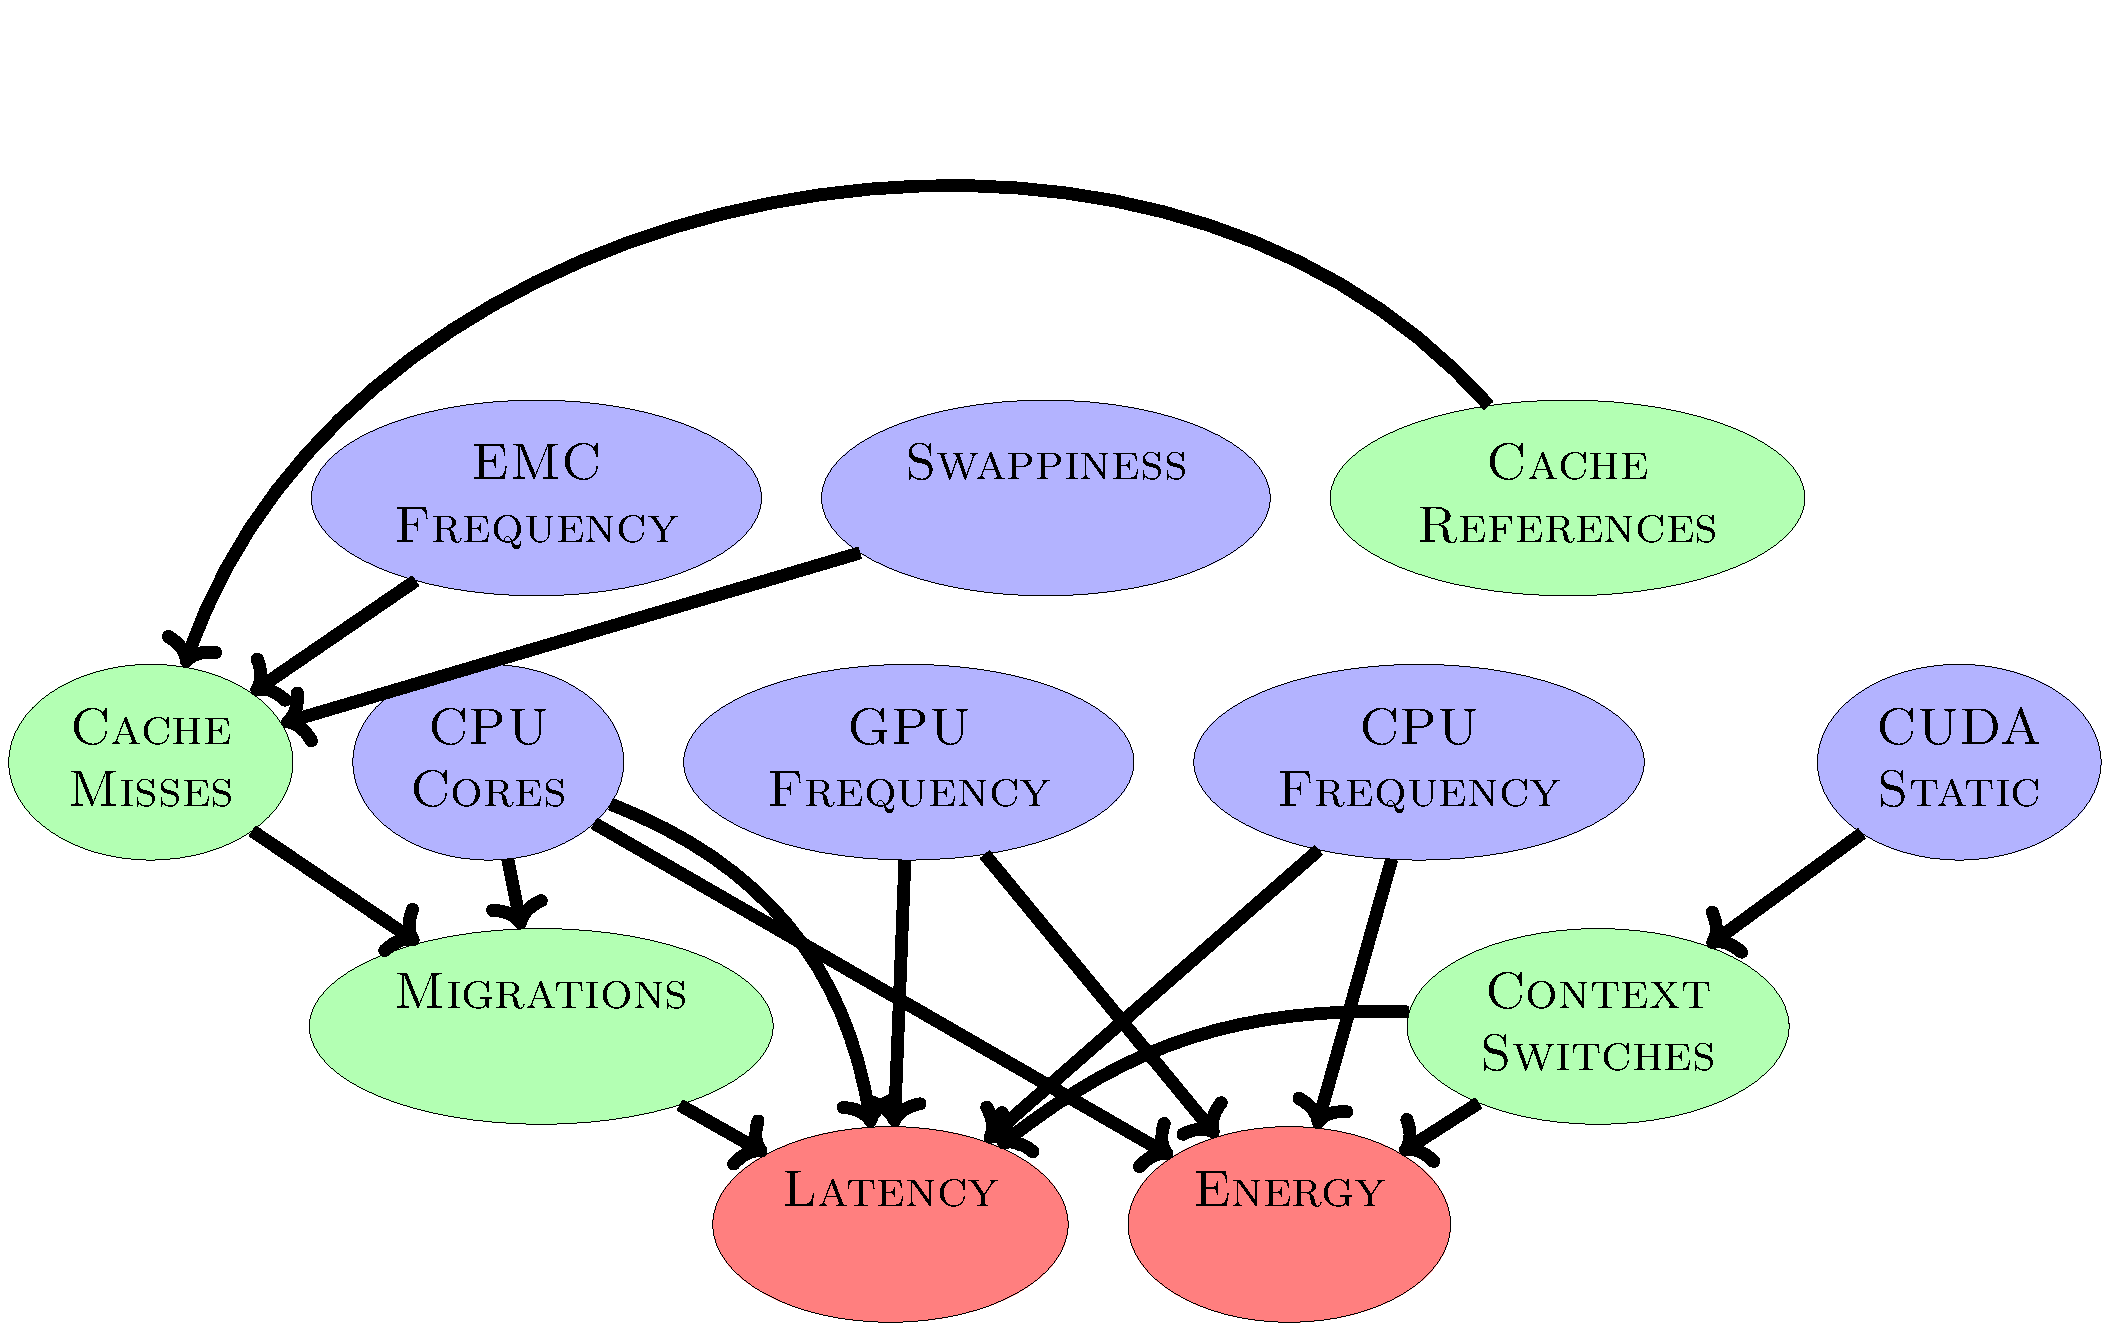
\includegraphics[width=\linewidth]{fig__realworld.pdf}

\caption{\small Using \ourapproach on a real-world performance issue.}
\label{fig:real_example}
\end{figure}

% There are various classes of causal models that can be used in \ourapproach. Each class of causal models has its assumptions (e.g., the existence of a confounder), different expressivity levels (e.g., capturing interactions), and they may impose some constraints (e.g., allowing hybrid variables including both discrete and continuous data). 

% For the experiments reported in this paper, we use \textit{acyclic directed mixed graph} (hereafter, ADMG), \ie, an acyclic graph consisting of directed and bidirected edges representing the causal direction and existence of latent common cause(s), respectively~\cite{richardson2002ancestral, evans2014markovian}. The nodes of the ADMG have the configuration options and the non-functional properties (\eg, latency, \, etc). Additionally, we enrich the causal graph by including nodes that represent the status of internal systems events, e.g., \textit{BranchMisses} in \fig{causal_model_example}. 

% It consists of configuration options set to {randomly} chosen values; various system events occurring when these configurations were used; and the measure of latency and energy. 

% \footnote{For our systems, we found that 25 initial samples were adequate to build an initial version of a causal model. However, this is a parameter that may change with the system.}
% \eg, resource pressure (as in~\fig{casusal_model_example}). Unlike configuration options, these system events cannot be modified. However, they can be observed and measured to explain how the causal-effect of changing configurations propagates to latency or energy, \eg, in~\fig{casusal_model_example} resource pressure is a system event that determines how \gpugrowth affects latency.


% We choose structural causal models as the basis of our formal discussion as they have the advantage of giving a sound foundation for various causal notions we will encounter. The easiest way to conceptualize a structural causal model is as a program for generating a distribution from independent noise variables through a sequence of formal instructions. Let’s unpack this statement. Imagine instead of samples from a distribution, somebody gave you a step-by-step computer program to generate samples on your own starting from a random seed. The process is not unlike how you would write code. You start from a simple random seed and build up increasingly more complex constructs. That is basically what a structural causal model is, except that each assignment uses the language of mathematics rather than any concrete programming syntax.



%As explained in \tion{cauper_help}, \texttt{DVFS} (a system event) dynamically scales the \texttt{core frequency} (a configurable option). This will have a proportionate effect on latency (a non-fuctional property we are interested in). Therefore, in order to understand the effect of \texttt{core frequency} on \texttt{latency}, we must account for the influence of \texttt{DVFS} in our model.

% \noindent{\textbf{Data collection.}}~

% FCI produces a \textit{partial acyclic graph} (hereafter, PAG) where some edges may not be oriented, \ie, they are undirected or partially directed. Below, we provide a brief overview of FCI. Next, we discuss how to orient its undirected and partially directed edges to produce an ADMG. 

% \subsubsection{Discovering causal structure with FCI}



% \noindent{\textbf{Structural causal model.}}~We construct a structural causal model (SCM using the observational data. SCM operates in three stages. First, we construct a fully connected undirected graph where each variable is connected to every other variable. Second, we use statistical independence tests to prune away edges between variables that are independent of one another. 

% \noindent{\textbf{Causal structure learning.}}~We use a structure discovery algorithm%, \eg, scheduler policy can be set to ``CFP'' or ``NOOP'' while dirty ratio can be set to any value from 1 to 100.


% To do this, for all pairs of variables say X and Y, we look for other variables say Z that can make X independent of Y when conditioned on Z. If we find any such variable, we remove the edge between X and Y, \ie, there is an edge between X and Y $\mathit{iff}$ they are dependent, regardless of what other variable it is being conditioned on. 

%More details about how to orient partially directed edges are in the appendix.

% , \ie, all three edges induce the same conditional independence relationships.



% \looseness=-1
% FCI operates in three stages. First, we build a skeleton graph that contains undirected edges from nodes that are dependent on each other.%; next, we orient undirected edges by applying a set of established edge orientation rules~\cite{spirtes2000causation}. 
% To build the skeleton graph, we first construct a fully connected undirected graph where each variable is connected to every other variable. Next, for every pair of variables X and Y, we look for other variables Z that can make X independent of Y when conditioned on Z. If we find any such variable, we remove the edge between X and Y, \ie, there is an edge between X and Y $\mathit{iff}$ we cannot make the dependence between them go away, regardless of what other variable its conditioned on. \tab{fci_example} shows a simple example with four variables $(W, X, Y, Z)$. Here, the first column depicts the fully connected graph. The column `independence' denotes the outcome of Fisher's exact independence test. In the column `Skeleton $(S)$', the independence results are used to prune edges from the fully connected graph. 
% After building the skeleton graph, FCI uses several rules\footnote{We do not discuss the orientation rules in detail here. These rules have been studied extensively, and we direct interested readers to works of Sprites~\etal~\cite{spirtes2000causation,ogarrio2016hybrid, glymour2019review} and Colombo~\etal~\cite{colombo2012learning,colombo2014order} for a thorough discussion on this topic.} to orient the undirected edges. FCI converts the undirected edges into 4 types shown in~\tab{edge_types}. Edge type 1 (\edgeone) indicates the direction of cause can be determined. Edge types 2 (\edgetwo) and 3 (\edgethree), indicate that the edge direction could be estimated but there is an uncertainty due to a possible hidden confounder. Finally, edge type 4 (\edgefour~) indicates that data is insufficient to detect the direction of causality. 


% \begin{table}[tbp!]
%     \centering
%     \caption{\small Description of edge types in the PAG generated by FCI.}
%     \label{tab:edge_types}
%     \resizebox{\linewidth}{!}{%
%     \begin{tabular}{rcl}
%         \hlineB{2}
%     Type & Edge & Description \bigstrut\\ \hlineB{2}
%     1 & A\edgeone ~B & A causes B \bigstrut\\ 
%     2 & A\edgetwo ~B & Unmeasured Confounder between A and B \bigstrut\\ 
%     3 & A\edgethree ~B & A causes B (or there are unmeasured confounders) \bigstrut\\ 
%     4 & A\edgefour ~B & Insufficient Data \bigstrut\\ \hlineB{2}
%     \end{tabular}%
%     }
% \end{table}

%If the threshold exceeds $1400$, we keep the edge, otherwise, we remove it.
% \fig{notears_samp} illustrates an example of an ADMG obtained with NOTEARS. The confidence scores are highlighted in \red{red}.  

% \begin{figure}[t!]
    \centering
    \subfloat[][FCI (PAG).]{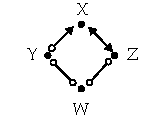
\includegraphics[width=0.3\linewidth]{fig__fci_sample_1.pdf}\label{fig:fci_samp}}
    %
    ~
    %
    \subfloat[][NOTEARS (DAG).]{\includegraphics[width=0.3\linewidth]{fig__notears_sample_1.pdf}\label{fig:notears_samp}}
    %
    ~
    %
    \subfloat[][Final ADMG.]{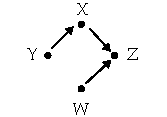
\includegraphics[width=0.3\linewidth]{fig__DAG_sample.pdf}\label{fig:dag_samp}}
    \caption{\small Resolving ties between FCI and NOTEARS.}
    \label{fig:ties}
\end{figure}

% We compare all the partially directed edges from the FCI's PAG (\fig{fci_samp_d}) with their corresponding counterparts from NOTEARS' DAG (\fig{fci_samp_e}). We experienced the following three contrasting edges between FCI and NOTEARS:
% \be[wide=0pt, topsep=0pt]
% \item \textit{\edgethree and \edgeone:} In the most common case, we observed that FCI had a partially directed edge and NOTEARS had a directed edge (as seen in the edge between \swapmem and \texttt{latency} in \Cref{fig:fci_samp_d,fig:fci_samp_e}). Here we kept the directed edge since evidence from NOTEARS provides us the directionality.
% \item  \textit{\edgefour~ and \edgeone:} In the second most common case, we observed FCI had an undirected edge and NOTEARS had a directed edge (as seen in the edge between \texttt{Resource} \texttt{Pressure} and \swapmem in \Cref{fig:fci_samp_d,fig:fci_samp_e}). Here again, we kept the directed edge in accordance with NOTEARS.
% \item \textit{\edgetwo and no edge:} Rarely, we observed that FCI had an undirected edge and NOTEARS had no edge (as seen in the edge between \gpugrowth and \swapmem in \Cref{fig:fci_samp_d,fig:fci_samp_e}). Here, we retain the bidirected edge since there likely is a latent confounder to be accommodated for.
% \ee
% %

% The final causal model would be an ADMG that resembles~\fig{fci_samp_f}. As discussed in~\tion{incremental_learning}, we update the observational data, and consequently the causal graph and the internal edge directions, periodically with new samples. %The rest of this section discusses how the causal model obtained above is used for subsequent analyses.

% \noindent\textbf{Why not use only NOTEARS?~}~We refrain from using only NOTEARS because it assumes that there are no unmeasured variables, \ie, strict causal sufficiency~\cite{lauer2017causal}. This is too restrictive since, there may be other variables that we cannot measure that may affect our observations, \eg, an increase in the environmental temperature may initiate the on-board thermal throttling fail-safe to dynamically reduce the clock speeds. FCI can accommodate such unmeasured confounders. 


% \paragraph{Phase-III: Translate Perf. Query to Causal Query}

\paragraph{Stage III: Iterative Sampling (Active Learning).}
\label{sect:path_discovery}

% In the previous stage, we convert unstructured observational data into structured ADMG. These ADMGs are still quite intricate and express several complex causal relationships among variables. 

% In this stage, we reason about the root causes of non-functional faults by: (1)~extracting the \textit{causal paths} from the ADMG and (2)~weighting the causal paths based on their average causal effect on the performance objectives. 

At this stage, \ourapproach determines the next configuration to be measured. 
\ourapproach first estimates the causal effects of configuration options towards performance objectives using the learned causal performance model. Then, \ourapproach iteratively determines the next system configuration using the estimated causal effects as a heuristic. Specifically, \ourapproach determines the value assignments for options with a probability that is determined proportionally based on their associated causal effects. The key intuition is that such changes in the options are more likely to have a larger effect on performance objectives, and therefore, we can learn more about the performance behavior of the system. Given the exponentially large configuration space and the fact that the span of performance variations is determined by a small percentage of configurations, if we had ignored such estimates for determining the change in configuration options, the next configurations would result in considerable variations in performance objectives comparing with the existing data. Therefore, measuring the next configuration would not provide additional information for the causal model. 

We extract paths from the causal graph (referred to as \textit{causal paths}) and rank them from highest to lowest based on their average causal effect on latency, and energy. Using path extraction and ranking, we reduce the complex causal graph into a few useful causal paths for further analyses. The configurations in this path are more likely to be associated with the root cause of the fault.

\noindent\textbf{Extracting causal paths with backtracking.}~A causal path is a directed path originating from either the configuration options or the system event and terminating at a non-functional property (\ie, throughput and/or energy). To discover causal paths, we backtrack from the nodes corresponding to each non-functional property until we reach a node with no parents. If any intermediate node has more than one parent, then we create a path for each parent and continue backtracking on each parent. 
% \eg, \cpufreq~\edgeone \util \edgeone Latency and  \cpucores~\edgeone \util \edgeone Latency. Since we can only intervene on configuration options we eliminate the paths that do not contain any configurations options \eg,  \contextswitches~\edgeone \cachepressure \edgeone Latency. %For example, from~\fig{fci_samp_f}, we can extract two paths:


\noindent\textbf{Ranking causal paths.~}~A complex causal graph can result in many causal paths. It is not practical to reason over all possible paths, as it may lead to a combinatorial explosion. Therefore, we rank the paths in descending of their causal effect on each non-functional property. For further analysis, we use paths with the highest causal effect.
% \label{sect:pace}
To rank the paths, we measure the causal effect of changing the value of one node (say \texttt{Batch Size} or $X$) on its successor (say \texttt{Cache Misses} or $Z$) in the path (say \texttt{Batch Size}~\edgeone \texttt{Cache Misses} \edgeone \texttt{FPS} and \texttt{Energy}). We express this with the \textit{do-calculus}~\cite{pearl2009causality} notation: $\mathbb{E}[Z~|~\mathit{do}(X=x)]$. This notation represents the expected value of $Z$ (\texttt{Cache Misses}) if we set the value of the node $X$ (\texttt{Batch Size}) to $x$. To compute the \textit{average causal effect} (ACE) of $X\rightarrow Z$ (\ie, \texttt{Batch Size} \edgeone \texttt{Cache Misses}), we find the average effect over all permissible values of $X$ (\texttt{Batch Size}), \ie, $\mathrm{ACE}\left(Z, X\right) = \frac{1}{N}\cdot \sum_{\forall a, b\in X}\mathbb{E}\left[Z~|~\mathit{do}\left(X=b\right)\right]~-~ \mathbb{E}\left[Z~|~\mathit{do}\left(X=a\right)\right]$.  Here $N$ represents the total number of values $X$ (\texttt{Batch Size}) can take. If changes in \texttt{Batch Size} result in a large change in \texttt{Cache Misses}, then $\mathrm{ACE}\left(Z, X\right)$ will be larger, indicating that \texttt{Batch Size} has a large causal effect on \texttt{Cache Misses}.

% {\footnotesize
% \begin{multline}
% \label{eq:ace}
% \mathrm{ACE}\left(Z, X\right) = \frac{1}{N}\cdot \sum_{\forall a, b\in X}\mathbb{E}\left[Z~|~\mathit{do}\left(X=b\right)\right]~-~ \mathbb{E}\left[Z~|~\mathit{do}\left(X=a\right)\right]
% \end{multline}
% }


% In this paper, we use K=3, 5,7, and 9, however, this may be modified in our replication package. 

% by carrying out the optimal intervention experiment predicted to cause the largest change in our belief (in expectation) and updating the belief. The final belief is summarized into a predicted network via Bayesian model averaging.




\paragraph{Stage IV: Update Causal Performance Model.}
\label{sect:incremental_learning}


% the estimations of causal queries act as a heuristic to select the next configuration to be measured to maximize the likelihood of improving the estimates 

At each iteration, \ourapproach measures the configuration that is determined in the previous stage and updates the causal performance model incrementally (shown in~\fig{causal_model_update}). 
Since the causal model uses limited observational data, there may be a discrepancy between the underlying performance model and the learned causal performance model, note that this issue exists in all domains using data-driven models, including causal reasoning~\cite{pearl2009causality}. The more accurate the causal graph, the more accurate the proposed intervention will be~\cite{spirtes2000causation,ogarrio2016hybrid, glymour2019review,colombo2012learning,colombo2014order}. \fig{incremental_update} (a) shows an example of an iterative decrease of hamming distance~\cite{norouzi2012hamming} between the learned causal model and (approximate) ground truth causal model. \fig{incremental_update} (b), \ref{fig:incremental_update} (c), and \ref{fig:incremental_update} (d) shows the iterative behavior of \ourapproach while debugging a multi-objective performance fault. In case our repairs do not fix the faults, we update the observational data with this new configuration and repeat the process. Over time, the estimations of causal effects will become more accurate. We terminate the incremental learning once we achieve the desired performance.

% The reason behind this initial sampling is to learn an initial causal model and given that our sampling budget is limited, we maximize the information in the causal model iteratively following a Bayesian approach where at iteration $t$ the current causal model is considered as prior and given the new sample it gets updated.



% \begin{figure}[t!]
%     % \setlength{\belowcaptionskip}{-3em}
%     \centering
%     \includegraphics*[width=\linewidth]{figures-vg/acc_shd_iter.pdf}
%     \caption{\small {}}
    
%     \label{fig:acc_shd_iter}
%     % \rayb{I have questions about this figure. Let's talk in the morning}
% \end{figure}


\paragraph{Stage V: Estimate Performance Queries.}
\label{sect:path_discovery}
At this stage, given the learned causal performance model, \ourapproach's inference engine estimates the user-specified queries using the mathematics of causal reasoning--do-calculus.
Specifically, the causal inference engine provides a quantitative estimate for the identifiable queries on the current causal model and may return some queries as unidentifiable. It also determines what assumptions or new measurements are required to answer the ``unanswerable`` questions, so, the user can decide to incorporate these new assumptions by defining more constraints or increasing the sampling budgets.

% \smallskip
% \paragraph{Implementation.}
% There are generic causal inference tools` maintained by industry (e.g., Microsoft's DoWhy~\cite{dowhy}, IBM's CausalLib~\cite{causalevaluations}, Uber's CausalML~\cite{causalml}), and academia (e.g., Ananke~\cite{ananke}, Causal Fusion~\cite{fusion}); these tools only implement the core machinery in causal reasoning including different causal modeling, structure learning, inference, counterfactuals, and estimation tasks. 
% We implemented \ourapproach by integrating and building on top of (i) \emph{Semopy}~\cite{semopy} for predictions with causal models, (ii) \emph{Ananke}~\cite{ananke} for estimating the causal effects, (iii) \emph{CausalML}~\cite{causalml} for counterfactual reasoning, \emph{PyCausal}~\cite{pycausal} for structure learning. 
% In particular, we integrated the tools into a seamless pipeline to provide users with the following capabilities for performance modeling and analyses: (i) \textbf{Modeling}: specifying the causal variables and constraints needed for learning a correct causal performance model (see Section \ref{sec:motivation}); (ii) \textbf{Analyses}: Iterative sampling, model learning and update, estimation of performance queries, and early stopping; and (iii) \textbf{User interface}: visualization, annotations, interactions with CPM models, and query estimations.

% \textcolor{blue}{To do so, we extract paths from the CPM (referred to as \textit{causal paths}) and rank them from highest to lowest based on their average causal effect (ACE) on performance objective. Using path extraction and ranking, we reduce the complex causal graph into a few useful causal paths for further analyses. The configurations in this path are more likely to be associated with the root cause of the fault.
% \noindent\textbf{Extracting causal paths with backtracking.}~A causal path is a directed path originating from either the configuration options or the system event and terminating at a non-functional property (\ie, throughput and/or energy). To discover causal paths, we backtrack from the nodes corresponding to each non-functional property until we reach a node with no parents. If any intermediate node has more than one parent, then we create a path for each parent and continue backtracking on each parent. 
% \eg, Batch Size~\edgeone Cache Misses \edgeone Throughput and En and  \cpucores~\edgeone \util \edgeone Latency. Since we can only intervene on configuration options we eliminate the paths that do not contain any configurations options \eg,  \contextswitches~\edgeone \cachepressure \edgeone Latency. %For example, from~\fig{fci_samp_f}, we can extract two paths:

% \bi[topsep=0pt] 
% \item \swapmem~\edgeone \gpugrowth \edgeone Latency; and
% \item Resource Pressure~\edgeone Latency
% \ei
% Note, there may be edges between two non-functional properties, \eg, latency\edgetwo energy. However, paths always terminate at a non-functional property, \ie, at latency, energy consumption, and heat dissipation.
% 

% \noindent\textbf{Ranking causal paths.~}~A complex causal graph can result in a large number of causal paths. It is not practical to reason over all possible paths as it may lead to a combinatorial explosion. Therefore, we rank the paths in descending of their causal effect on each non-functional property. For further analysis, we use paths with the highest causal effect.
% % \label{sect:pace}
% To rank the paths, we measure the causal effect of changing the value of one node (say \textsc{Vm Swappiness} or $X$) on its successor (say \textsc{Cache Load Misses} or $Z$) in the path (say \textsc{VM Swappiness}~\edgeone \textsc{Cache Load Misses} \edgeone \textsc{Latency} and \textsc{Energy}). We express this with the \textit{do-calculus}~\cite{pearl2009causality} notation: $\mathbb{E}[Z~|~\mathit{do}(X=x)]$. This notation represents the expected value of $Z$ (\textsc{Cache Load Misses}) if we set the value of the node $X$ (\textsc{VM Swappiness}) to $x$. To compute the \textit{average causal effect} (ACE) of $X\rightarrow Z$ (\ie, \textsc{VM Swappiness} \edgeone \textsc{Cache Load Misses}), we find the average effect over all permissible values of $X$ (\textsc{VM Swappiness}), \ie, 

% {\footnotesize
% \setlength{\abovedisplayskip}{1pt}
% \setlength{\belowdisplayskip}{1pt}
% \begin{multline}
% \label{eq:ace}
% \mathrm{ACE}\left(Z, X\right) = \frac{1}{N}\cdot \sum_{\forall a, b\in X}\mathbb{E}\left[Z~|~\mathit{do}\left(X=b\right)\right]~-~ \mathbb{E}\left[Z~|~\mathit{do}\left(X=a\right)\right]
% \end{multline}
% }

% Here, $N$ represents the total number of values $X$ (\textsc{VM Swappiness}) can take. If changes in \textsc{VM Swappiness} result in a large change in \textsc{Cache Load Misses}, then the $\mathrm{ACE}\left(Z, X\right)$ will be larger, indicating that \textsc{VM Swappiness} on average has a large causal effect on \textsc{Cache Load Misses}. %Note, if $X$ is a continuous variable, we would replace the summation of \eq{ace} with an integral. 
% % 
% % \eq{ace} represents the average causal effect over a pair of nodes in a path. 
% For the entire path, we extend \eq{ace} as:
% \smalleq
% \label{eq:path_ace}
% {\footnotesize
% \setlength{\abovedisplayskip}{1pt}
% \setlength{\belowdisplayskip}{1pt}
% \mathrm{Path}_{ACE} = \frac{1}{K} \cdot \sum \mathrm{ACE}(Z, X) \hspace{2em} \footnotesize \forall X, Z \in path 
% }
% \eeq
% \eq{path_ace} represents the average causal effect of the causal path. The configuration options that lie in paths with larger $P_{ACE}$ tend to have a greater causal effect on the corresponding non-functional properties in those paths. We select the top $K$ paths with the largest $\mathrm{P}_{ACE}$ values, for each non-functional property. In this paper, we use K=5, however, this may be modified in our replication package. 

% \noindent\textbf{\textsl{Aside.}}~In eqs.~\ref{eq:do} and~\ref{eq:ace}, $\mathbb{E}(Y~|~do(X=x))$ is \textit{not} the same as the ordinary conditional distribution $\mathbb{E}\left(Y~|~X=x\right)$. This is because $\mathbb{E}\left(Y~|~X=x\right)$ takes the original population, as is, and filters it get the sub-population where $X=x$. If $X=x$ does not exist in the population, the value of $\mathbb{E}\left(Y~|~X=x\right)$ would be misleading. In contrast, $\mathbb{E}\left(Y~|~\mathit{do}\left(X=x\right)\right)$ uses do-calculus rules~\cite{pearl2009causality} to infer the value of the distribution even when $X=x$ has never been encountered before. 

% \subsubsection{Phase-III: Counterfactual Query Evaluation}
% \label{sect:root_cause}
% Counterfactual queries can be different for different tasks. For debugging, we use the top $K$ paths to (a)~identify the root cause of non-functional faults; and (b)~prescribe ways to fix the non-functional faults.
% % \subsubsection{Translating developer's queries into counterfactual statements}
% When experiencing non-functional faults, a developer may ask specific queries to \tool and expect an actionable response. We use the example causal graph of Fig.~\ref{fig:complex} where a developer observes high latency and energy, \ie, a multi-objective fault, and has the following questions:  %We use this example to answer some of the developer's questions: 

% \noindent\textbf{\faQuestionCircle~\textbf{``What are the root causes of my multi-objective (latency and energy) fault?''}} To identify the root cause of a non-functional fault we must identify which configuration options have the most causal effect on the performance objective. %For example, in the causal graph of~\fig{path_eg}, we are required to find which of the configuration options $X_1, X_2, Z_1, Z_2$ has the highest causal effect on $Y$. 
% For this, we use the steps outlined in~\tion{path_discovery} to extract the paths from the causal graph and rank the paths based on their average causal effect (\ie, $\mathrm{Path}_{ACE}$ from \eq{path_ace}) on latency and energy. We return the configurations that lie on the top $K$ paths. 
% For example, in~\fig{fci_samp_f} we may return (say) the following paths: 
% \bisq
% \small
%     \item \textsc{VM Swappiness}~\edgeone \textsc{Cache Load Misses} \edgeone \textsc{Latency} and \textsc{Energy}
%     \item  \textsc{Scheduler Policy} \edgeone \textsc{Branch Misses} \edgeone \textsc{Cache Misses} \edgeone \textsc{Latency} and \textsc{Energy}
%     \item  \textsc{Gpu Frequency} \edgeone \textsc{Latency} and \textsc{Energy}
%     \item  \textsc{Bit Rate} \edgeone \textsc{Cache Misses} \edgeone \textsc{Latency} and \textsc{Energy}
%     \item  \textsc{Scheduler Runtime} \edgeone \textsc{Branch Misses} \edgeone \textsc{Cache Misses} \edgeone \textsc{Latency} and \textsc{Energy}
% \ei
 
% % \item \cpufreq~\edgeone \swapmem \edgeone Latency,
% and the configuration options {\textsc{VM Swappiness}, \textsc{Scheduler Policy}, \textsc{Gpu Frequency}, \textsc{Bit Rate}, \textit{and} \textsc{Scheduler Runtime}} being the probable root causes.

% \noindent\textbf{\faQuestionCircle~\textbf{``How to improve my latency and energy?''}} To answer this query, we first find the root causes as described above. Next, we discover what values each of the configuration options must take so that the new latency and energy are better (low latency and low energy) than the fault (high latency and high energy). For example, we consider the causal path \textsc{VM Swappiness}~\edgeone \textsc{Cache Load Misses} \edgeone \textsc{Latency} and \textsc{Energy}, we identify the permitted values for the configuration options {\textsc{VM Swappiness}} that can result in a low latency and energy ($Y^{\mathit{\textsc{low}}}$) that is better than the fault ($Y^{\mathit{\textsc{high}}}$).
% For this, we formulate the following counterfactual expression: 
% \smalleq
% \label{eq:cfact_bare}
% \footnotesize
% \mathrm{Pr}(Y_{repair}^{\textsc{low}}|\neg repair,Y_{\neg repair}^{\textsc{high}})
% \eeq
% \eq{cfact_bare} measures the probability of ``fixing'' the latency fault with a ``repair'' {\footnotesize $(Y_{repair}^{\textsc{low}})$} given that with no repair {we observed the fault} {\footnotesize $(Y_{\neg repair}^{\text{\textsc{high}}})$}.   
% In our example, the repairs would resemble \textsc{VM Swappiness}=$0.6$ \etc. We generate a \textit{repair set} ($\mathcal{R}_{1}$), where the configurations \textsc{VM Swappiness} is set to all permissible values, \ie,
% {
% \small
% \begin{multline}\label{eq:repairs}
%     \setlength{\abovedisplayskip}{5pt}
%     \setlength{\belowdisplayskip}{5pt}
%     \mathcal{R}_{1}\equiv~\bigcup~\left\{\textsc{VM Swappiness} = {x},... \right\}\forall {x} \in \textsc{Vm Swappiness},~\ldots
% \end{multline}}
% Observe that, in the repair set ($\mathcal{R}_{1}$) a configuration option that is not on the path \textsc{VM Swappiness}~\edgeone \textsc{Cache Load Misses} \edgeone \textsc{Latency} and \textsc{Energy} is set to the same value of the fault. For example, \textsc{Active Cores} is set to $2$ or \textsc{Gpu Frequency} is set to $0.7 \ GHz$. This way we can reason about the effect of interactions between \textsc{VM Swappiness} with other options, i.e., \textsc{Active Cores}, \textsc{Gpu Frequency}. Say \textsc{Active Cores} or \textsc{Gpu Frequency} were changed/recommended to set at any other value than the fault in some previous iteration i.e., $3$ or $1.5 \ GHz$, respectively. In that case, we set \textsc{Active Cores} and \textsc{Gpu Frequency}=$1.5 \ GHz$. Similarly, we generate a repair sets $\mathcal{R}_{2}$ to $\mathcal{R}_{5}$  by setting \textsc{Scheduler Policy}, \textsc{Gpu Frequency}, \textsc{Bit Rate} and \textsc{Scheduler Runtime} to all permissible values. 
% {
% \small
% \begin{multline}\label{eq:repairs}
%     \setlength{\abovedisplayskip}{5pt}
%     \setlength{\belowdisplayskip}{5pt}
%     \mathcal{R}_{2}\equiv~\bigcup~\left\{\textsc{Scheduler Policy} = {x},... \right\} \forall {x} \in \textsc{Scheduler Policy},~\ldots
% \end{multline}}
% {
% \small
% \begin{multline}\label{eq:repairs}
%     \setlength{\abovedisplayskip}{5pt}
%     \setlength{\belowdisplayskip}{5pt}
%     \mathcal{R}_{3}\equiv~\bigcup~\left\{\textsc{Gpu Frequency} = {x},... \right\} \forall {x} \in \textsc{Gpu Frequency},~\ldots
% \end{multline}} 
% {
% \small
% \begin{multline}\label{eq:repairs}
%     \setlength{\abovedisplayskip}{5pt}
%     \setlength{\belowdisplayskip}{5pt}
%     \mathcal{R}_{4}\equiv~\bigcup~\left\{\textsc{Bit Rate} = {x},... \right\} \forall {x} \in \textsc{Bit Rate},~\ldots
% \end{multline}} 
% {
% \small
% \begin{multline}\label{eq:repairs}
%     \setlength{\abovedisplayskip}{5pt}
%     \setlength{\belowdisplayskip}{5pt}
%     \mathcal{R}_{5}\equiv~\bigcup~\left\{\textsc{Scheduler Runtime} = {x},... \right\} \forall {x} \in \textsc{Scheduler Runtime},~\ldots
% \end{multline}} 
% Now, we combine the repair set for each path to construct a final repair set $\mathcal{R}=\mathcal{R}_{1} \cup~\ldots \cup\mathcal{R}_{k}$. Next, we compute the \textit{individual treatment effect} (ITE) on the latency and energy ($Y$) for each repair in the repair set $\mathcal{R}$. In our case, for each repair $\mathit{r}~\in~\mathcal{R}$, ITE is given by:
% \begin{equation}
%     \label{eq:ite}
%     \footnotesize
%     \mathrm{ITE}(\mathit{r})=\mathrm{Pr}(Y_r^{\textsc{low}}~|~\neg r,~Y_{\neg r}^{\textsc{high}}) - \mathrm{Pr}(Y_r^{\textsc{high}}~|~\neg r,~Y_{\neg r}^{\textsc{high}})\hspace{1em}
% \end{equation}

% % The above formulation can be extended to accommodate queries that involve multiple non-functional properties (\eg, improve \textit{both} latency and energy consumption). To do this, we may reformulate \eq{ite} to compute the probability that a repair $r$ can reduce both latency ($Y_r^{\textsc{low}}$) and the energy consumption ($W_r^{\textsc{low}}$), \ie,
% % {
% % \small
% % \begin{multline}\label{eq:repairs_2}
% %     \setlength{\abovedisplayskip}{5pt}
% %     \setlength{\belowdisplayskip}{5pt}
% %     \mathrm{ITE}(\mathit{r})=\mathrm{Pr}(Y_r^{\textsc{low}}, W_r^{\textsc{low}}~|~\neg r,~Y_{\neg r}^{\textsc{high}},~W_{\neg r}^{\textsc{high}}) \\ -~\mathrm{Pr}(Y_r^{\textsc{high}}, W_r^{\textsc{high}}~|~\neg r,~Y_{\neg r}^{\textsc{high}},~W_{\neg r}^{\textsc{high}})
% % \end{multline}}
% % \noindent\hspace{-3pt}After, computing \eq{repairs_2}, we can find a repair $r$ with the largest (positive) ITE as per~\eq{best_intervention}. 
% % \begin{equation}
% %     \label{eq:ite}
% %     \footnotesize
% %     \mathrm{ITE}(\mathit{r})=\mathrm{Pr}(Y_r^{\textsc{low}}, W_r^{\textsc{low}}~|~\neg r,~Y_{\neg r}^{\textsc{high}},~W_{\neg r}^{\textsc{high}}) - \mathrm{Pr}(Y_r^{\textsc{high}}~|~\neg r,~Y_{\neg r}^{\textsc{low}})\hspace{1em}
% % \end{equation}

% % \[\bigcup\limits_{{x_1} \in {X_1},{x_2} \in {X_2},...} {P(Y = {y_{fixed}}|do({X_1} = {x_1},{X_2} = {x_2},...))} \]

% % \noindent\textbf{\faQuestionCircle~\textbf{``How to decrease my latency using the same energy consumption''}} There queries involve multiple non-functional properties (in this case, latency and energy consumption). 
% % % An example, let us try to minimize latency without affecting energy consumption. 
% % We enumerate all possible repairs as counterfactual statements as per~\eq{repairs}. Next, we compute the \textit{individual treatment effect} (ITE) for each repair in three steps: 
% % \besq
% % \item  
% % {\footnotesize$\mathrm{P_{fix}}=\mathrm{Pr}(Y_r^\textsc{low},~W_r^\textsc{same}~|~\neg r,W_{\neg r}^\textsc{same}, Y_{\neg r}^\textsc{high} )$}.
% % \item Compute the probability that a repair $r$ \textit{cannot} fix the latency (\ie, $Y^{\text{\textsc{high}}}$) or it actually worsens energy consumption (\ie, $W^{\text{\textsc{high}}}$), \ie, {\footnotesize$\mathrm{P_{no~fix}}=\mathrm{Pr}(W_r^\textsc{high},~Y_r^\textsc{high} ~|~\neg r,W_{\neg r}^\textsc{high}, Y_{\neg r}^\textsc{high})$}.
% % \item Finally, compute the $ITE(\mathit{r})$ as {$
% % \footnotesize \mathrm{ITE}(\mathit{r})=\mathrm{P_{fix}} - \mathrm{P_{no~fix}}$}
% % \ee

% % If this difference is large, then the repair `$r$' has a high likelihood of fixing the latency fault in $Y^\text{\textsc{high}}$ while keeping the energy consumption $W^\text{\textsc{high}}$ unchanged.  We find the best repair operator with the highest $ITE(\mathit{r})$ using~\eq{best_intervention}. 

% \subsubsection*{Remarks.}~The ITE computation of \eq{ite} occurs \textit{only} on the observational data. Therefore we may generate any number of repairs and reason about them without having to deploy those interventions and measuring their performance in the real world. This offers significant runtime benefits.
% }
% If the new configuration addresses the \nfp, we return the recommended repairs to the developer. 



% We do not offer theoretical upper bounds for the convergence of the causal model. We shall address this in our future work. That said, our empirical evidence shows that our models converge after at most 50 additional samples.

% \subsection{Limitations of \tool}
% No tool is perfect, \tool is no exception. The efficacy of \tool depends on several factors such as the representativeness of the observational data or the presence of unmeasured confounders that negatively affect the quality of the causal model. An incorrect causal model may lack some crucial connections that may result in detecting spurious root causes or recommending incorrect repairs. One promising direction to address this problem would be to refine the causal model with developer feedback. Alternatively, we could transfer a causal model certified by experts for one domain to another equivalent domain. We shall explore these in future work. 

% \tool uses a query engine to translate common user queries into counterfactual statements. The query translation framework described in this section may be extended to answer more complex queries involving several more configurations and non-functional properties by reformulating the counterfactual expressions in~\eq{cfact_bare}. As part of our future work, we hope to develop a formal translation framework (\eg, in the form of a DSL) that can convert any user-provided query into a meaningful counterfactual statement. 


%%%%%% OLD %%%%%%%%
% \subsubsection{{Orienting undirected edges of the PAG from FCI}}

% We use NOTEARS \cite{zheng2018dags}, and an unconstrained optimization-based structural learning algorithm to learn a directed acyclic graph (DAG) from observational data. NOTEARS is useful for our application because it produces \textit{confidence scores} for each direction of edge orientation. We may this use to orient the partial edges. 


% Given observational data with (say) four variables $(W, X, Y, Z)$, NOTEARS learns a weighted adjacency matrix $A$. The weights determine the confidence that an edge exists between any two nodes (variables), \eg, $\left(A_{XY}=0.9, A_{YX}=0.1\right)$ indicates the confidence that there is an edge $X$\raisebox{1pt}{\edgeone}~$Y$ is 90\% while the confidence that there is an edge $Y$\raisebox{1pt}{\edgeone}~$X$ is only 10\%. 

% To generate a DAG, NOTEARS learns an adjacency matrix from the observational data. NOTEARS initializes an adjacency matrix $A$ with random values (between 0 and 1). Next, it defines a smooth function ($h$) that measures the ``DAG-ness'' of the graph such that $h(A)=0$ $\mathit{iff}$ the adjacency matrix $A$ is acyclic. Finally, it uses an unconstrained optimization to update the values of the adjacency matrix until the adjacency matrix converges. The final adjacency matrix has values that lie between 0 and 1, where 1 indicates high confidence that there is an edge and 0 otherwise.
% The directionality of the edge may be determined using the confidence scores, \eg, if $\mathit{confidence(}X$\raisebox{1pt}{\edgeone}~$Y)<\mathit{confidence}(Y$\raisebox{1pt}{\edgeone}~$X)$, then the edge directionality is $Y$\raisebox{1pt}{\edgeone}~$X$ (as seen in the edge between Resource Pressure and \swapmem in~\fig{fci_samp_e}).

% We obtain a DAG from the NOTEARS adjacency matrix to complement the PAG from FCI. This is done by setting a threshold on the confidence scores in the adjacency matrix. If the confidence of an edge in the adjacency matrix exceeds this threshold, we keep the edge otherwise we remove the edge, \eg, absent (grayed out) edge between \gpugrowth and \swapmem in~\fig{fci_samp_e}. The chosen threshold determines how many edges are retained. If the threshold is too low, then there will be a lot of spurious edges. Alternately, if the threshold is too high, the ADMG will be sparse. For this work, we found empirically that a threshold of $0.75$ for the confidence scores represented a reasonable balance. 
